\begin{figure}[tbph]
  \centering
  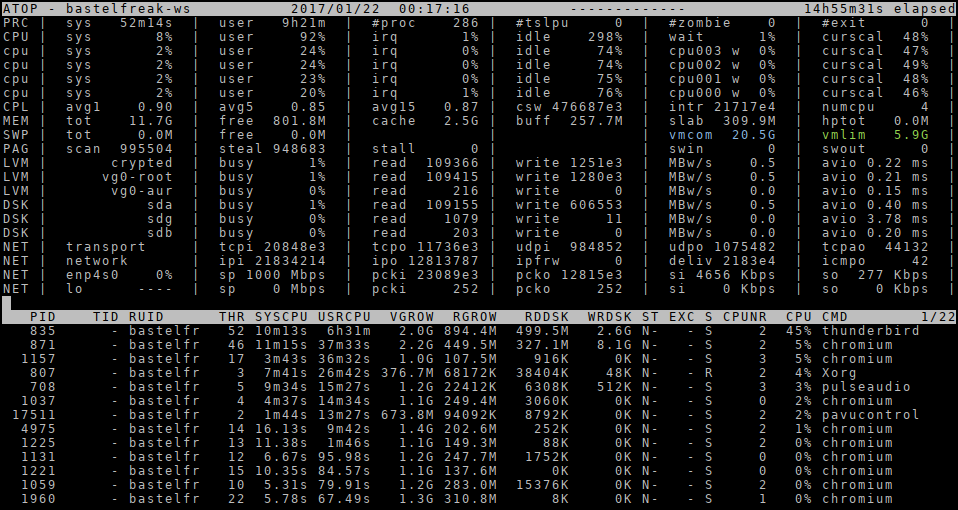
\includegraphics[width=1.0\textwidth]{../figures/atop_1.png}
  \caption{atop mit geringer Systemlast}
\label{figure:atop1}
\end{figure}

\begin{figure}[tbp]
  \centering
  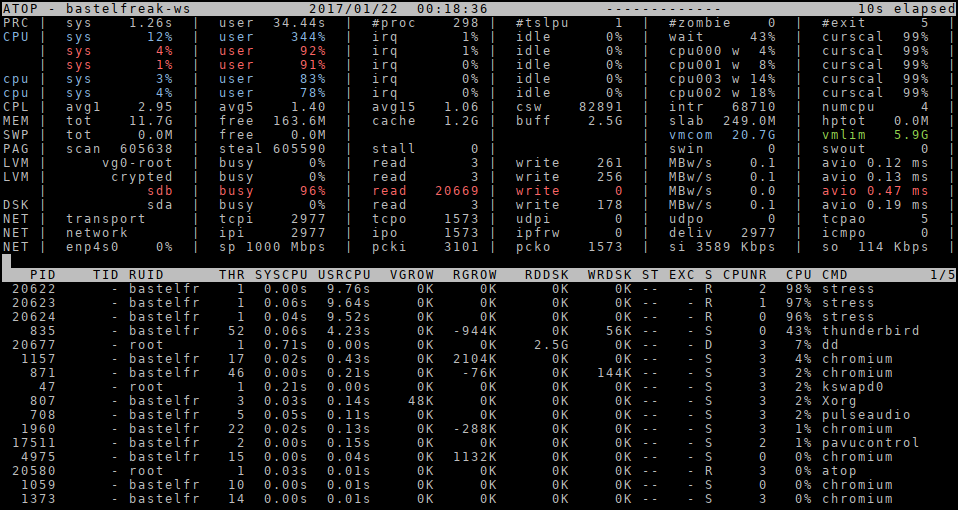
\includegraphics[width=1.0\textwidth]{../figures/atop_2.png}
  \caption{atop mit hoher CPU/Netzwerk Last}
\label{figure:atop2}
\end{figure}

\begin{figure}[tbp]
  \centering
  
\includegraphics[width=1.0\textwidth]{../figures/diamond.png}
  \caption{Offene PRs und Issues im Diamond Projekt am 22.01.2017}
\label{figure:diamond}
\end{figure}

\begin{figure}[tbp]
  \centering
%%  \includesvg[svgpath=../figures/,path=../figures/]{messagebusv1}
  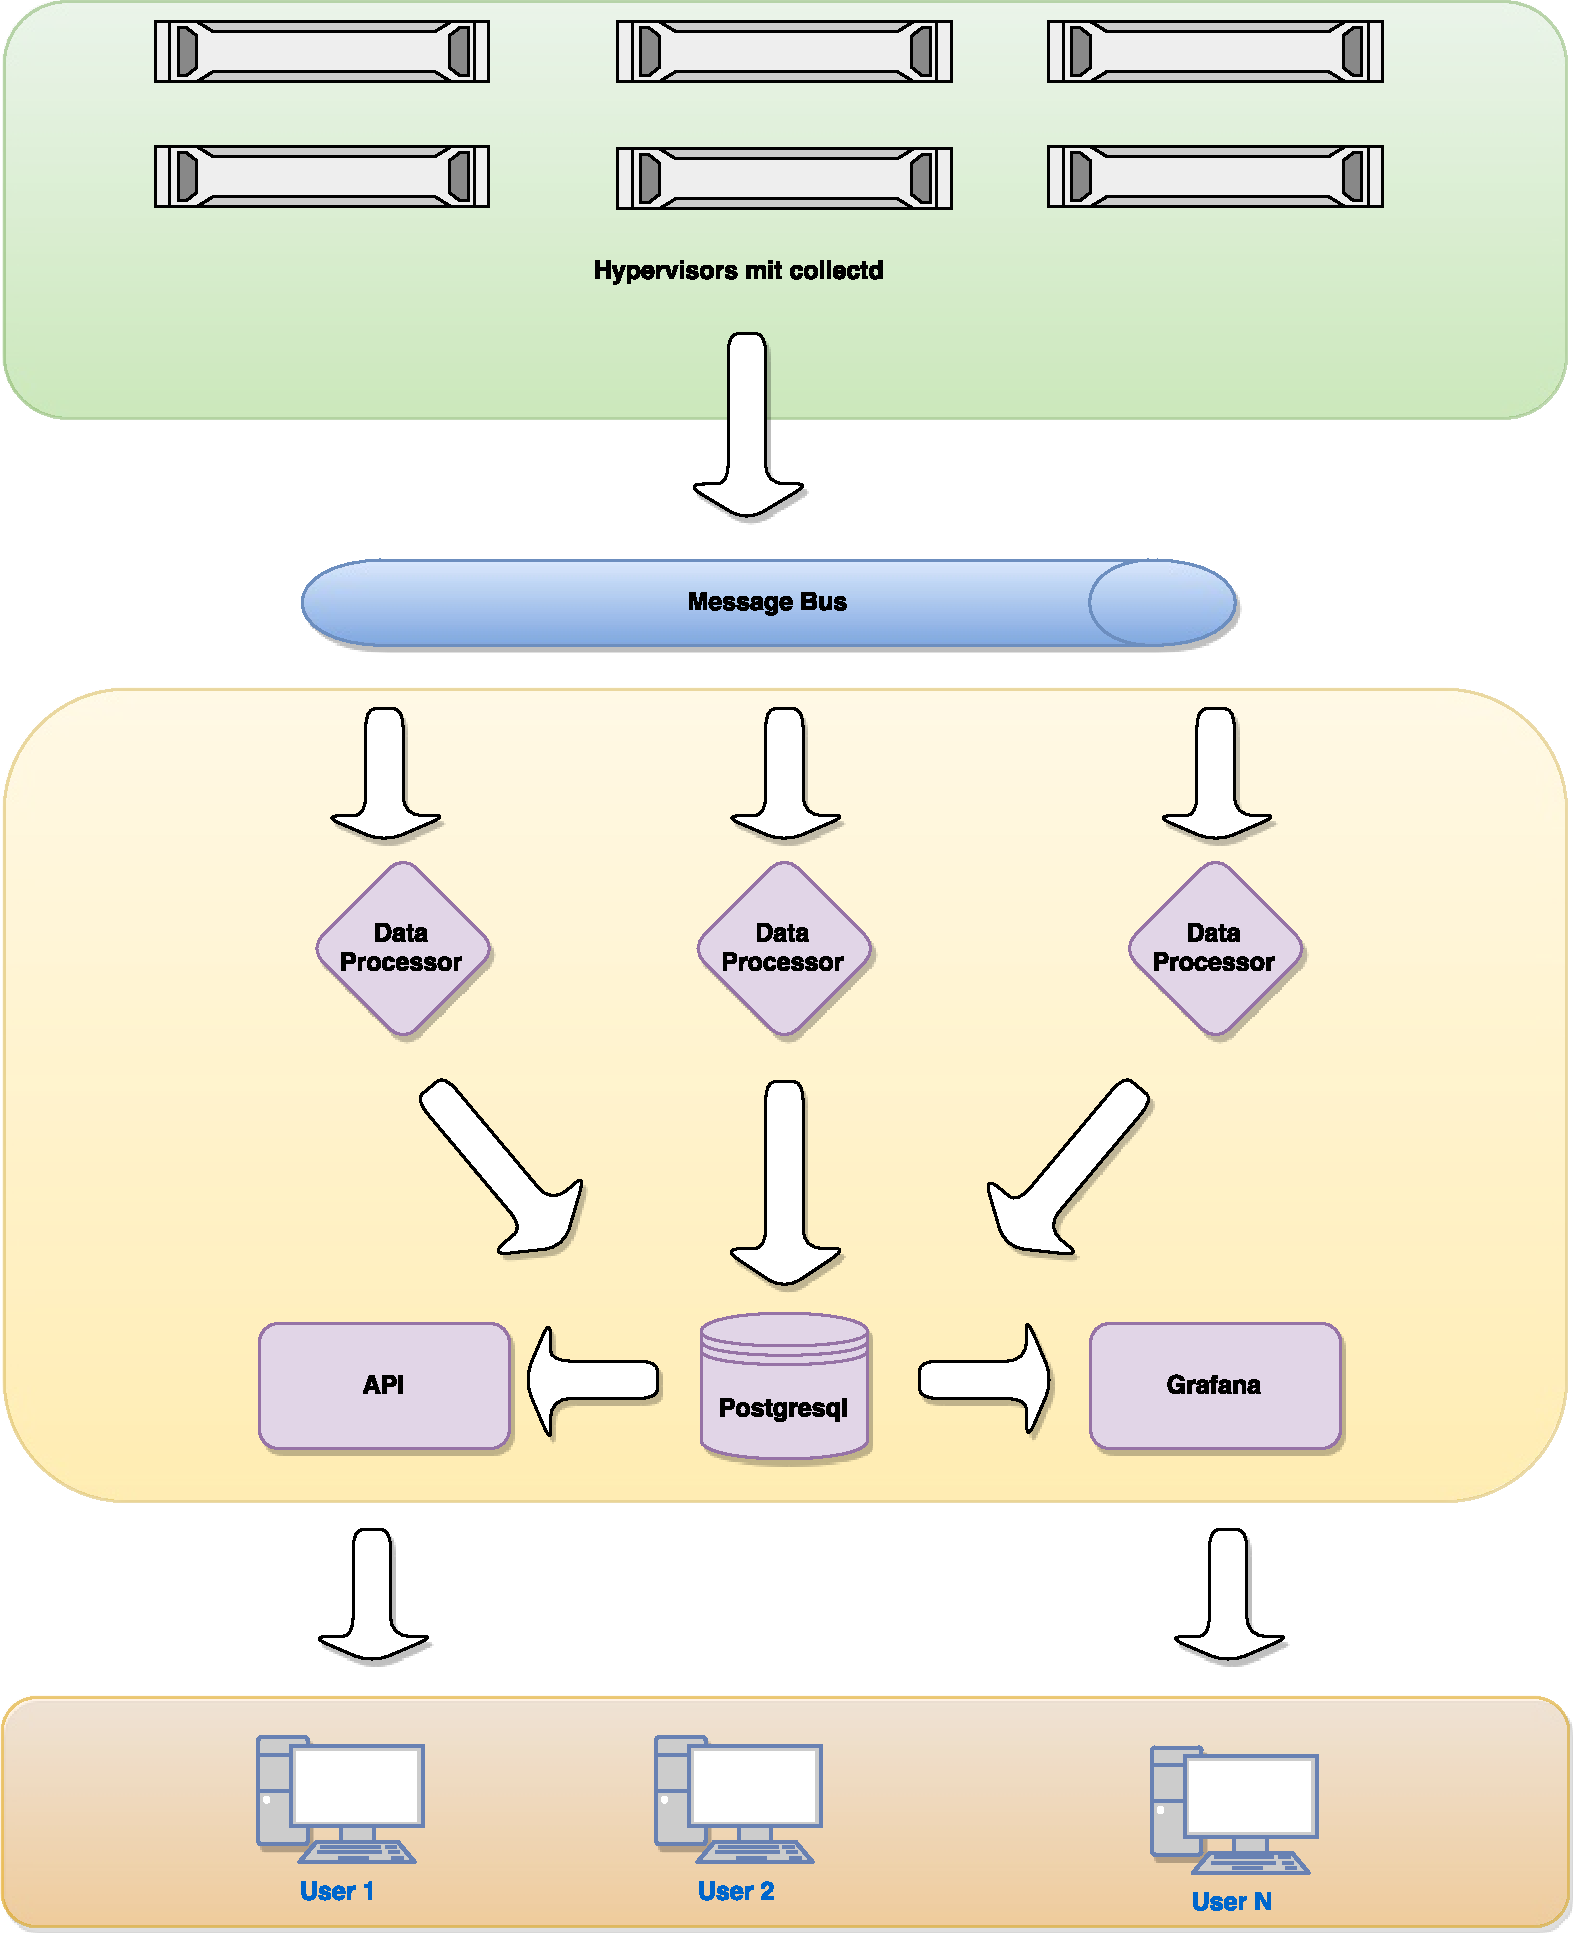
\includegraphics[width=1.0\textwidth]{../figures/messagebusv1_1.pdf}
  \caption{Architekturdraft Version 1}
\label{figure:draft1}
\end{figure}
\begin{figure}[tbp]
  \centering
%%  \includesvg[svgpath=../figures/,path=../figures/]{messagebusv1}
  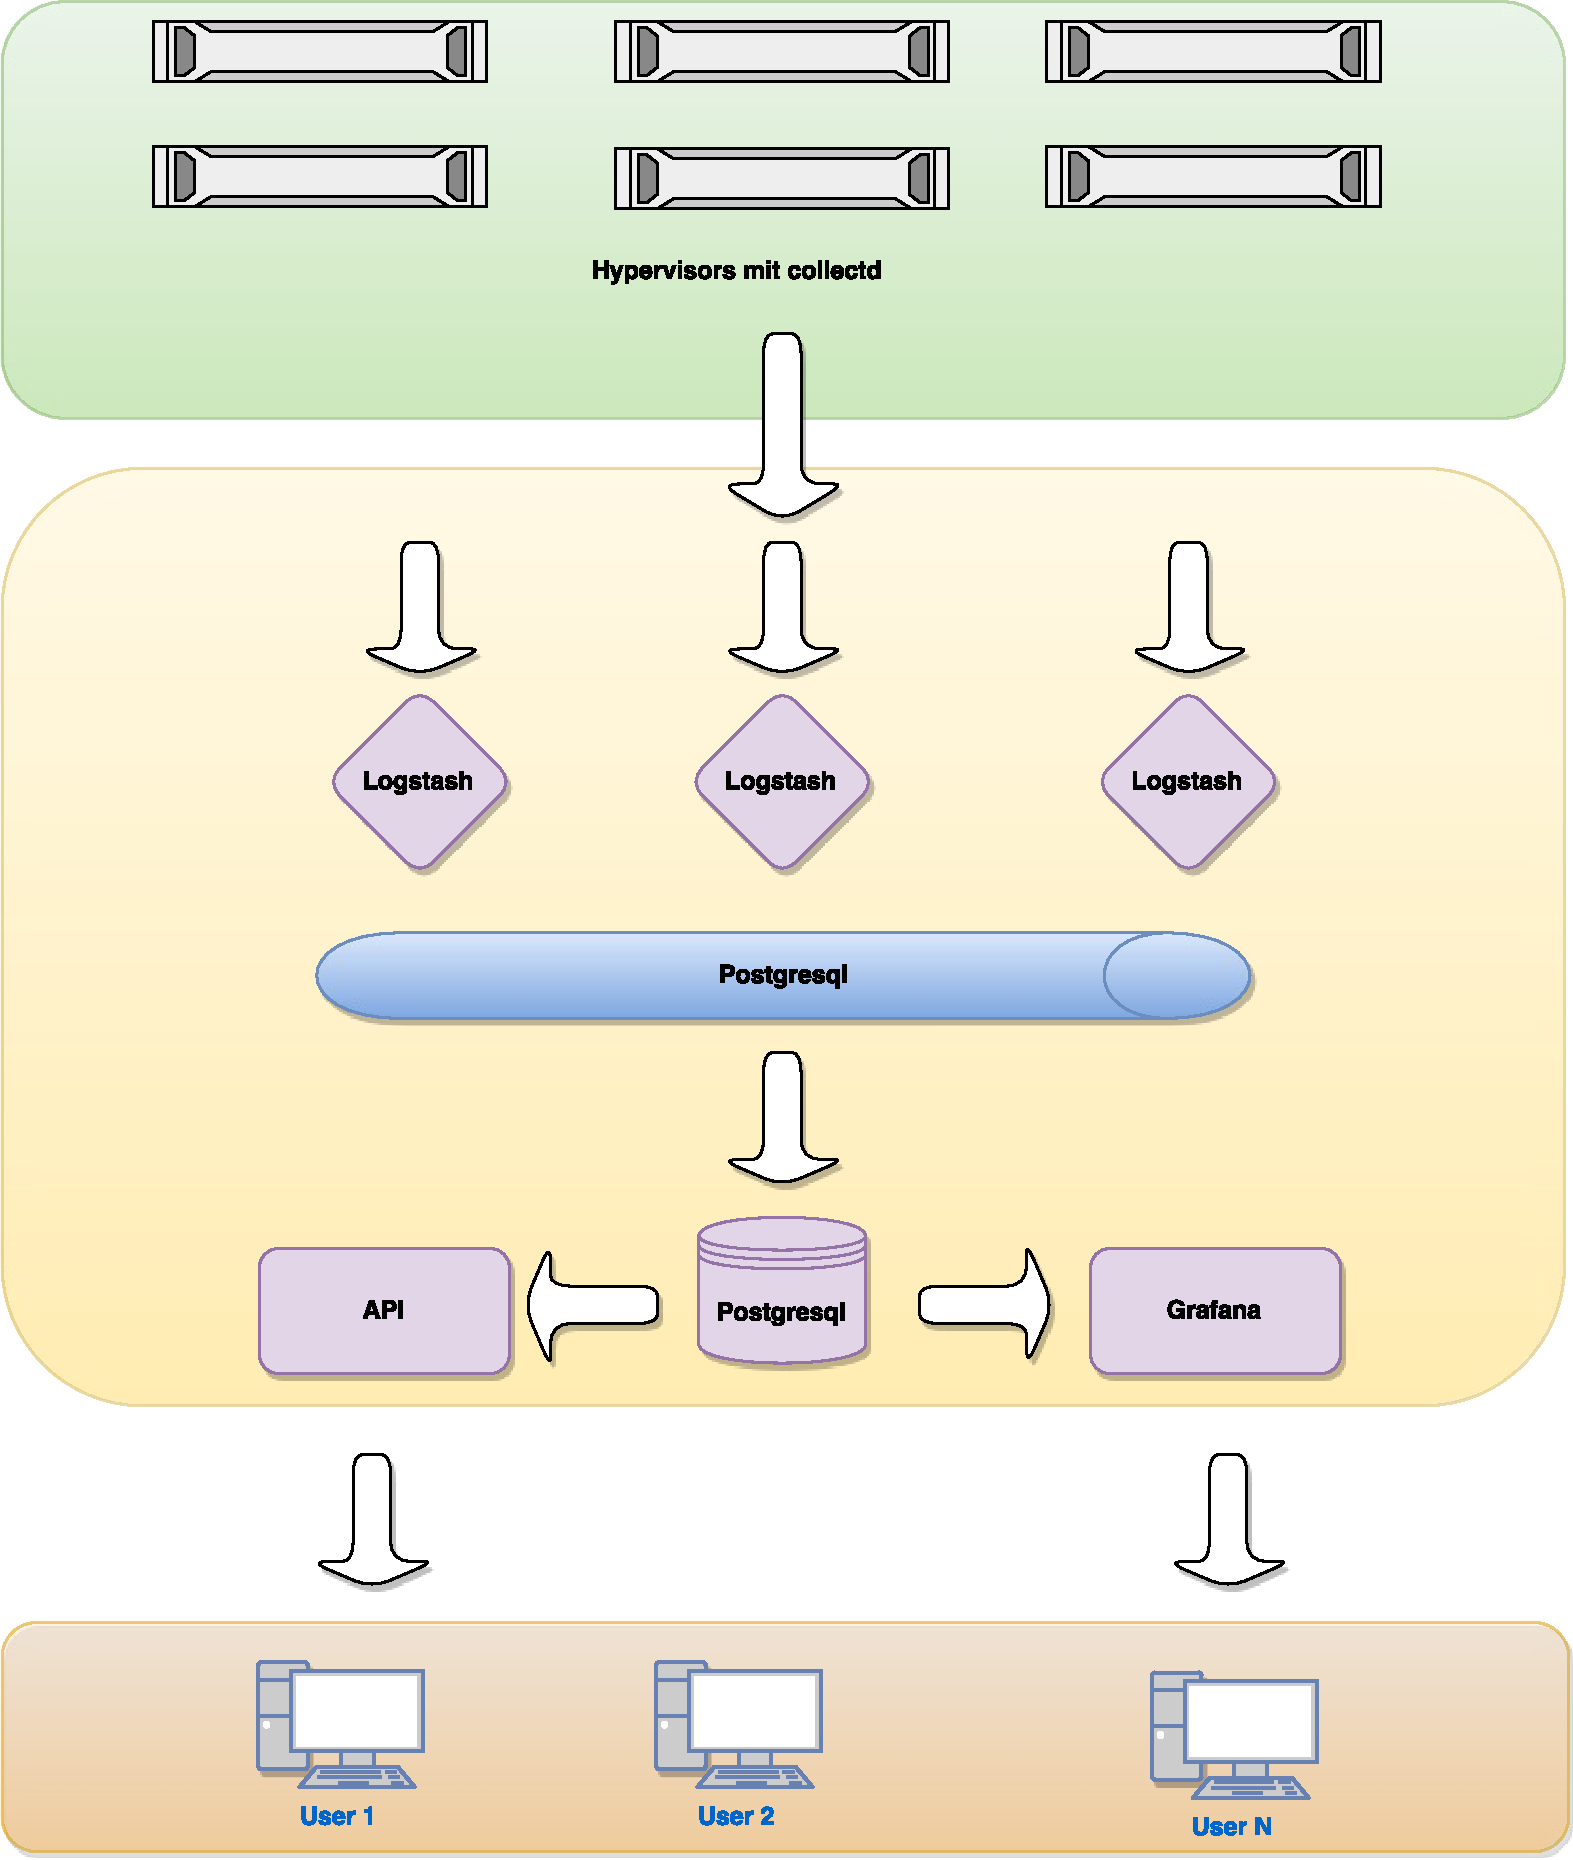
\includegraphics[width=1.0\textwidth]{../figures/messagebusv2_1.pdf}
  \caption{Architekturdraft Version 2}
\label{figure:draft2}
\end{figure}
\FloatBarrier{}

\begin{figure}[tbp]
  \centering
  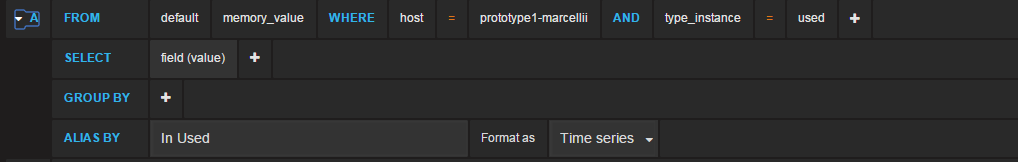
\includegraphics[width=1.0\textwidth]{../figures/graph.png}
  \caption{Beispielabfrage für eine Graphen Visualisierung}
\label{figure:graph}
\end{figure}

\begin{figure}[tbp]
  \centering
  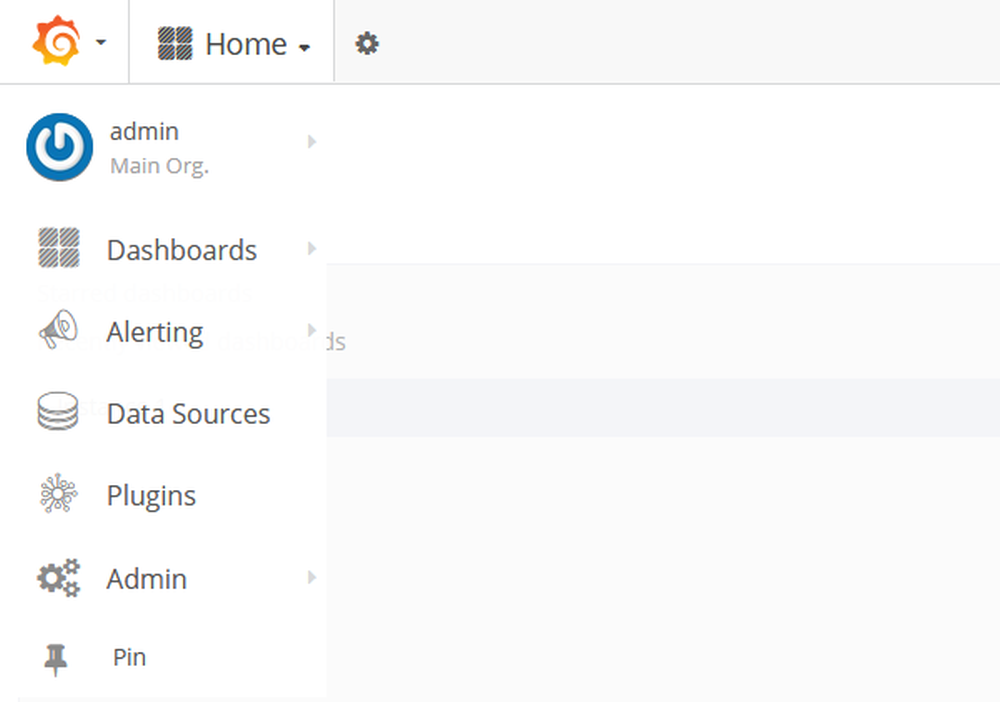
\includegraphics[width=1.0\textwidth]{../figures/grafana_dashboard_l.png}
  \caption{Grafana Dashboard Linke Seite}
\label{figure:grafana_dashboard_l}
\end{figure}

\begin{figure}[tbp]
  \centering
  
\includegraphics[width=1.0\textwidth]{../figures/grafana_dashboard_r.png}
  \caption{Grafana Dashboard Rechte Seite}
\label{figure:grafana_dashboard_r}
\end{figure}


